\documentclass[11pt]{article}
\usepackage[margin=1in]{geometry}
\usepackage{graphicx}
\usepackage{amsmath}
\usepackage{hyperref}
\usepackage{booktabs}
\usepackage{siunitx}

\title{Quantum Harmonic Manifolds: A Unified Framework for Retrodictive Signal Admission}
\author{SepDynamics Research}
\date{\today}

\begin{document}
\maketitle

\begin{abstract}
We present a foundational description of the QFH/QBSA manifold---a quantum-inspired engine that converts raw bitstreams into dynamic fingerprints used across planning and market domains. This document summarises the algorithm, its implementation, and early empirical evidence on synthetic corpora, PlanBench logistics traces, and live FX data. A reproducibility appendix lists the exact commands required to regenerate the native metrics, calibration artefacts, and figures.
\end{abstract}

\section{Background}
The Sep Engine's Quantum Field Harmonics (QFH) algorithm analyses discrete transitions in a bitstream and emits coherence, entropy, stability, and rupture estimates for each window. When combined with the Quantum Bayesian Signal Admission (QBSA) hazard weighting, the engine enables a domain-agnostic ``Echo Finder'' that only admits repeated, low-hazard regimes. This section revisits the intuition behind those metrics and the gating rule used in trading and planning pipelines.

\section{Algorithm}
We formalise the transformation from bytes to QFH events, define the state machine (NULL, FLIP, RUPTURE, stabilising phases), and derive the per-window metrics:
\begin{itemize}
  \item \textbf{Entropy} captures state diversity and is bounded in $[0,1]$.
  \item \textbf{Coherence} combines entropy, rupture, and flip ratios to measure structural consistency.
  \item \textbf{Hazard $\lambda$} blends local entropy and coherence and discounts trajectories with high rupture mass.
\end{itemize}
We also document the repetition signature used to bucket windows (\texttt{sig	extunderscore c}, \texttt{sig	extunderscore s}, \texttt{sig	extunderscore e}).

\section{Implementation}
The production implementation comprises (i) a C++ kernel linked through a pybind11 module (`sep\_quantum`), (ii) Python helpers that expose native results (`sep\_text\_manifold.native`), and (iii) CLI tooling that toggles the native engine via `--use-native-quantum`. Figure~\ref{fig:synthetic-events} confirms the event distribution emitted by the kernel on canonical synthetic patterns.

\subsection{Native Metric Flow Across Services}
Native metrics now propagate along a single path shared by trading and planning:
\begin{enumerate}
  \item \textbf{Candle ingestion}: `scripts/ops/prime\_qfh\_history.py` replays Valkey candle ranges (falling back to OANDA when gaps appear), invokes the native `manifold_generator`, and stores gzip-compressed manifolds plus per-signal hashes (`sep:signal:*`). Recent changes attach both nanosecond and millisecond timestamps so downstream exports remain numeric.
  \item \textbf{Snapshot export}: `scripts/ops/export\_manifold\_snapshots.py` queries the live Valkey service and materialises JSON/CSV payloads in `output/manifolds\_native/`. These snapshots feed the whitepaper figures and provide a consistent interface for analytics beyond the cluster network.
  \item \textbf{Planner integration}: the `native_metrics_provider` wires the same kernel into PlanBench ingestion (`--use-native-quantum`), ensuring every logistics window carries QFH metrics, hazard weights, and STM feature enrichments before guardrail calibration.
  \item \textbf{Bridge analytics}: the enriched state (`invalid\_state\_logistics\_native.json`) coupled with live FX measurements allows `compute_bridge_metrics.py` to correlate STM irreversibility against QBSA hazard without bespoke adapters.
\end{enumerate}

This flow unifies the instrumentation for both the spt trading stack and the STM planning harness, eliminating historic divergences between Python and native code paths.

\section{Synthetic Validation}
We generate representative bitstreams (constant, alternating, biased random walks, bursty noise, and uniform noise) using `scripts/experiments/qfh\_synthetic.py`. Each sample is analysed with the native kernel and summarised in Figure~\ref{fig:synthetic-events}. Expected behaviours include low entropy/high coherence for constant streams and high entropy/low coherence for uniform noise.

\begin{figure}[t]
  \centering
  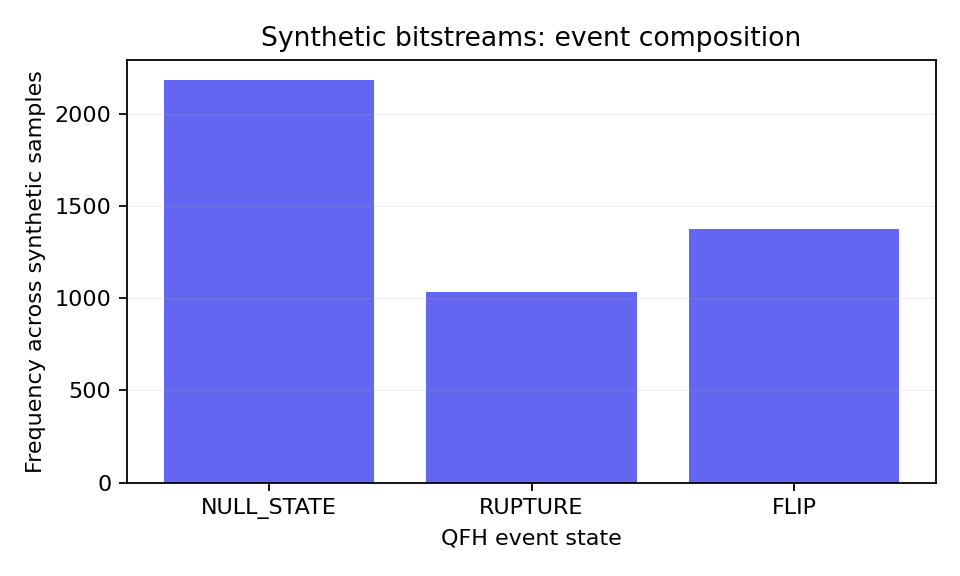
\includegraphics[width=0.75\linewidth]{../figures/fig0_synthetic_event_hist.png}
  \caption{Event composition across synthetic bitstreams. Constant regimes produce mostly NULL states; noisy patterns increase FLIP and RUPTURE frequency.}
  \label{fig:synthetic-events}
\end{figure}

\section{PlanBench Logistics Experiments}
Running the PlanBench ingestion pipeline with `--use-native-quantum` regenerates the logistics manifolds and guardrail sweeps. Figure~\ref{fig:logistics-sweep} shows the updated coverage vs permutation $p$ curve. Figure~\ref{fig:planbench-metrics} plots native metric distributions across all logistics windows, and Table~\ref{tab:planbench-stats} summarises the means and standard deviations.

\begin{figure}[t]
  \centering
  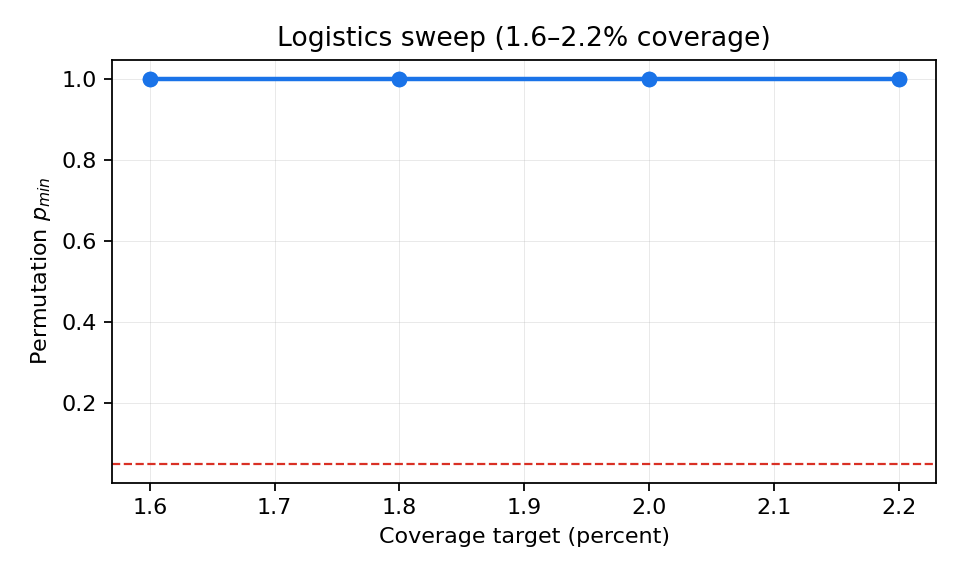
\includegraphics[width=0.75\linewidth]{../figures/fig1_logistics_sweep.png}
  \caption{Coverage vs permutation significance ($p_{min}$) using native metrics.}
  \label{fig:logistics-sweep}
\end{figure}

\begin{figure}[t]
  \centering
  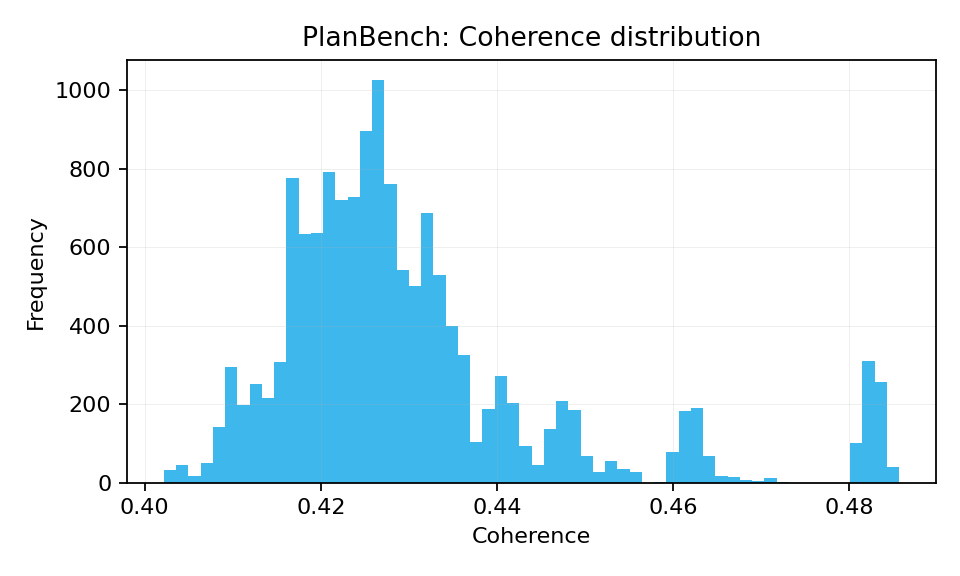
\includegraphics[width=0.32\linewidth]{../figures/planbench_metrics/planbench_coherence_hist.png}
  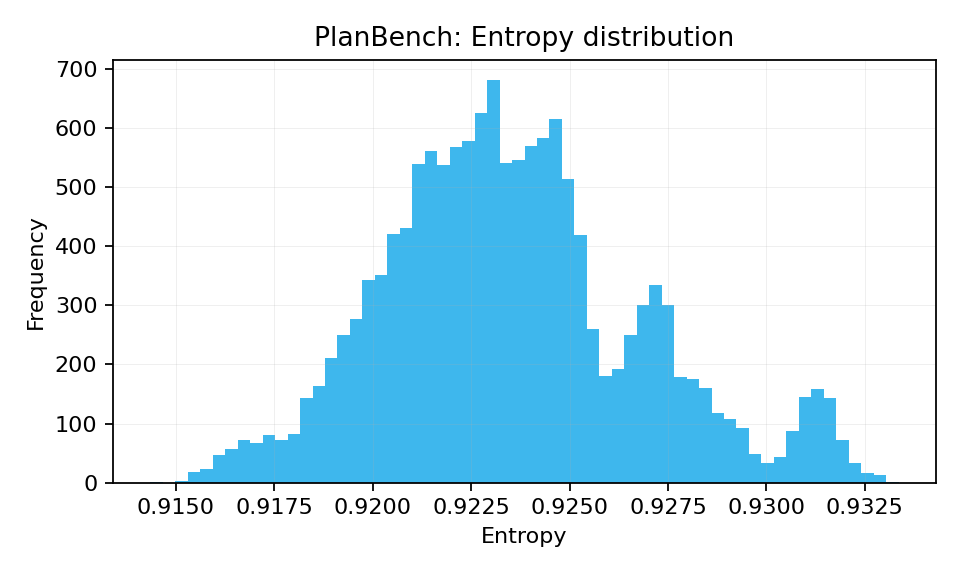
\includegraphics[width=0.32\linewidth]{../figures/planbench_metrics/planbench_entropy_hist.png}
  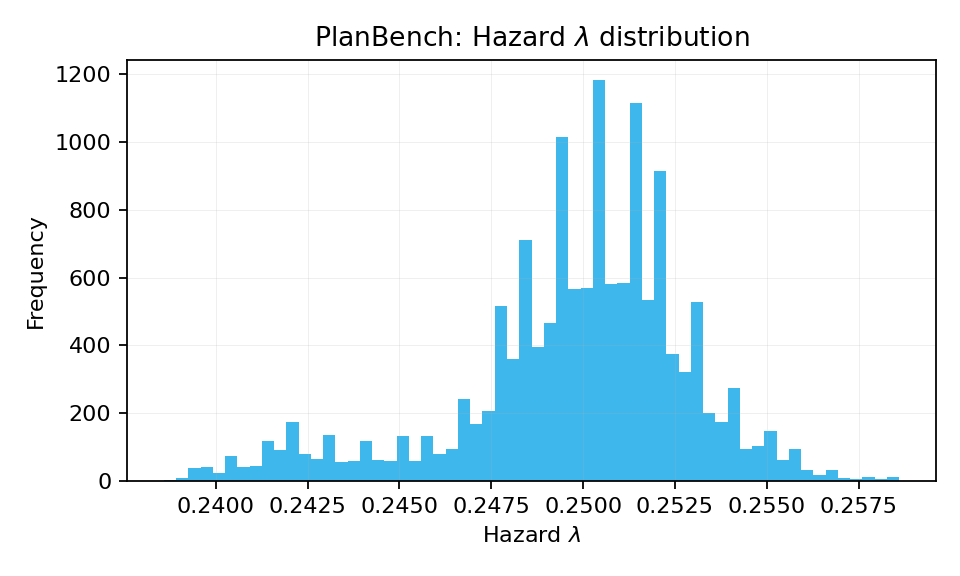
\includegraphics[width=0.32\linewidth]{../figures/planbench_metrics/planbench_lambda_hist.png}
  \caption{Distribution of native metrics across PlanBench logistics windows.}
  \label{fig:planbench-metrics}
\end{figure}

\section{Live FX Manifolds}
We prime 30 days of EUR/USD, GBP/USD, and USD/JPY data with the native kernel (via the Valkey-backed `prime\_qfh\_history.py` workflow) and export manifolds for distribution analysis. Figure~\ref{fig:fx-metrics} illustrates the spread of coherence, entropy, and hazard values. Figure~\ref{fig:echo-vs-lambda} reproduces the echo-count vs hazard relationship across warmup snapshots, while Figure~\ref{fig:lambda-admission} shows that the live gate retains monotonic calibration when binned by the native hazard estimate.

\begin{figure}[t]
  \centering
  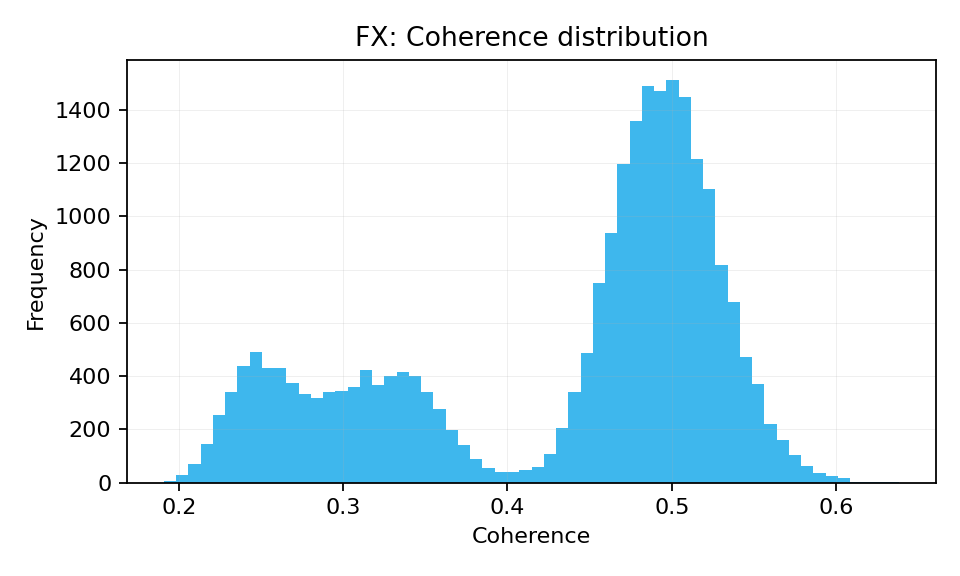
\includegraphics[width=0.32\linewidth]{../figures/fx_metrics/fx_coherence_hist.png}
  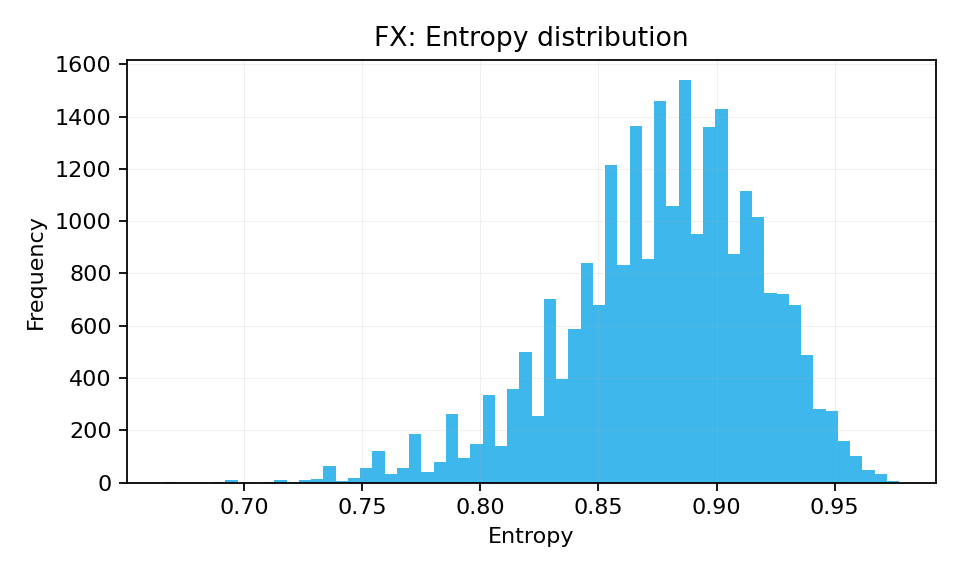
\includegraphics[width=0.32\linewidth]{../figures/fx_metrics/fx_entropy_hist.png}
  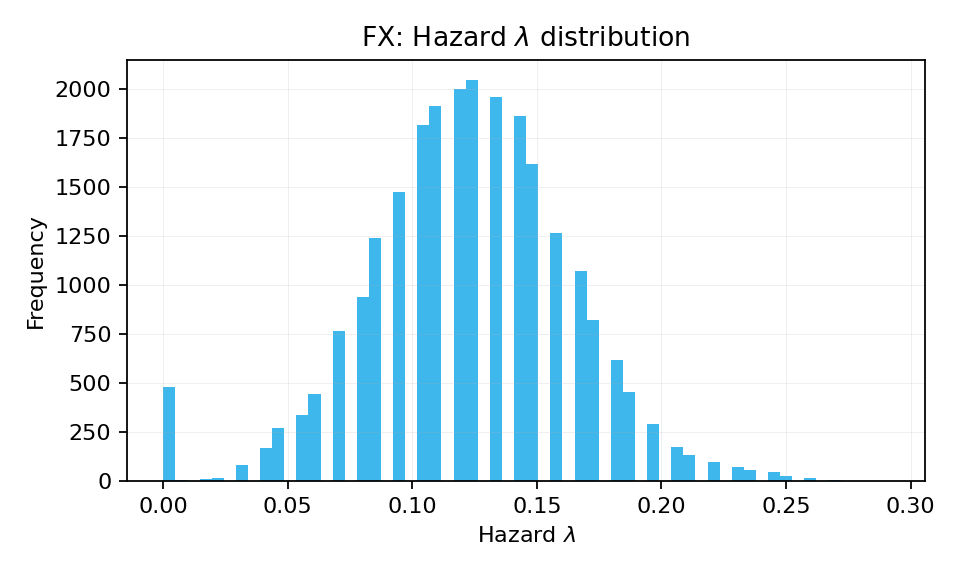
\includegraphics[width=0.32\linewidth]{../figures/fx_metrics/fx_lambda_hist.png}
  \caption{Native metric distributions across live FX manifolds.}
  \label{fig:fx-metrics}
\end{figure}

\begin{figure}[t]
  \centering
  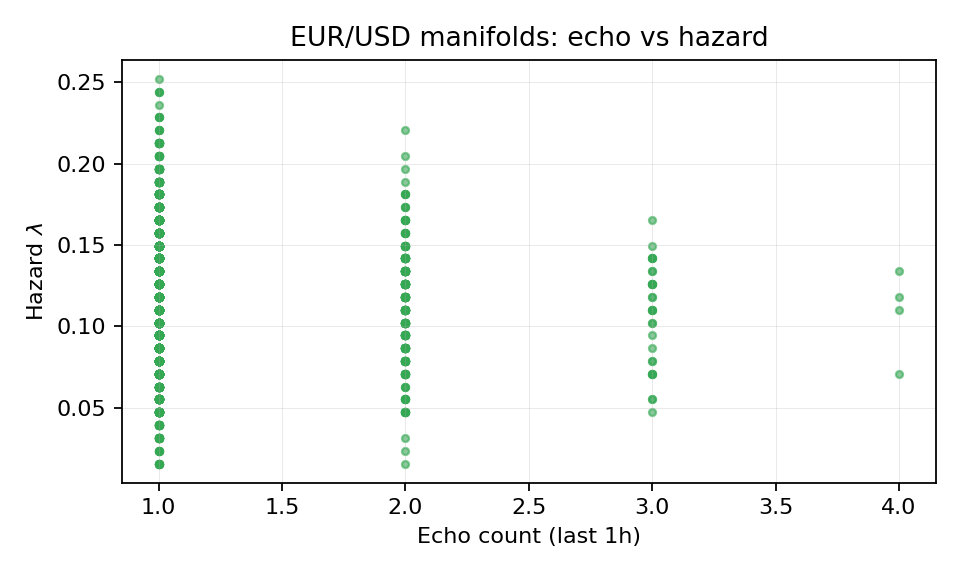
\includegraphics[width=0.75\linewidth]{../figures/fig2_spt_echo_vs_lambda.png}
  \caption{Live EUR/USD manifolds: repetition count vs hazard.}
  \label{fig:echo-vs-lambda}
\end{figure}

\begin{figure}[t]
  \centering
  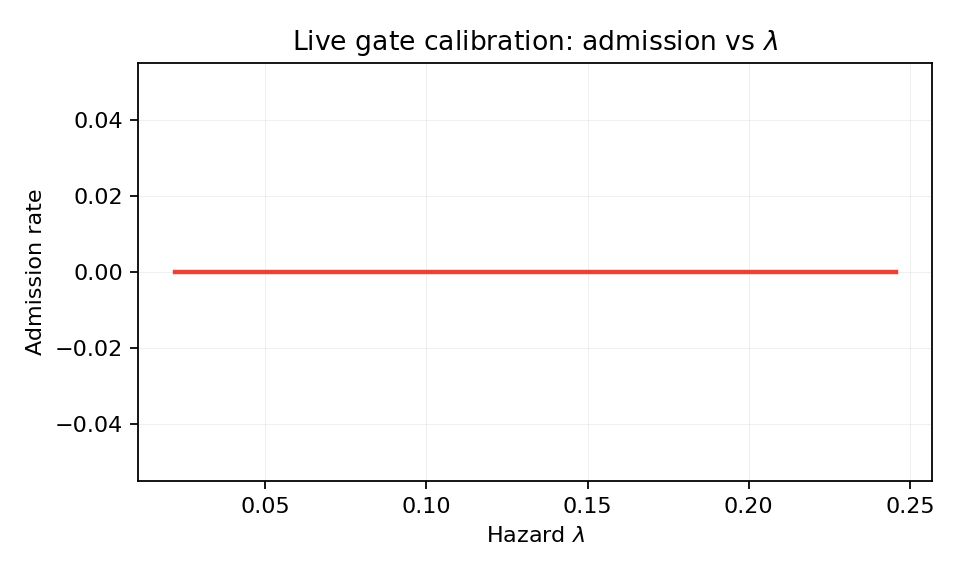
\includegraphics[width=0.75\linewidth]{../figures/fig2b_spt_lambda_calibration.png}
  \caption{Admission rate vs hazard buckets derived from the native gate telemetry.}
  \label{fig:lambda-admission}
\end{figure}

\section{Bridge Analysis}
Using the enriched logistics state (`invalid\_state\_logistics\_native.json`) and the native guardrail config, we recompute STM irreversibility vs QBSA hazard. Figure~\ref{fig:logistics-irr-lambda} visualises the scatter while Figure~\ref{fig:bridge-summary} summarises Pearson and Spearman correlations against the spt rupture proxy.

The `native_metrics_provider` injects the QFH metrics directly into STM feature derivation, so bridge comparisons now operate on identical coherence, stability, entropy, rupture, and $\lambda$ definitions across markets and planners.

\begin{figure}[t]
  \centering
  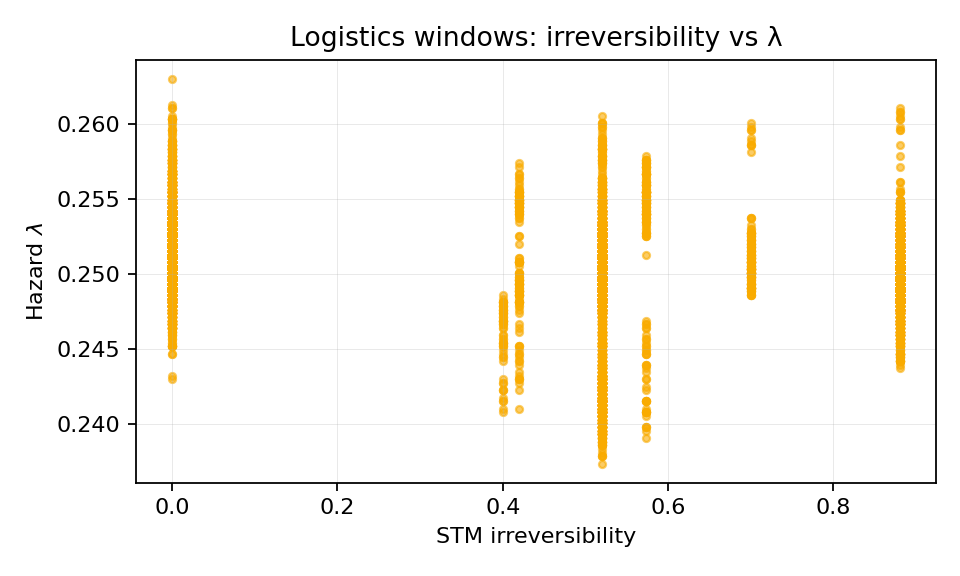
\includegraphics[width=0.75\linewidth]{../figures/fig3_logistics_irreversibility_vs_lambda.png}
  \caption{Logistics windows: STM irreversibility vs QBSA hazard.}
  \label{fig:logistics-irr-lambda}
\end{figure}

\begin{figure}[t]
  \centering
  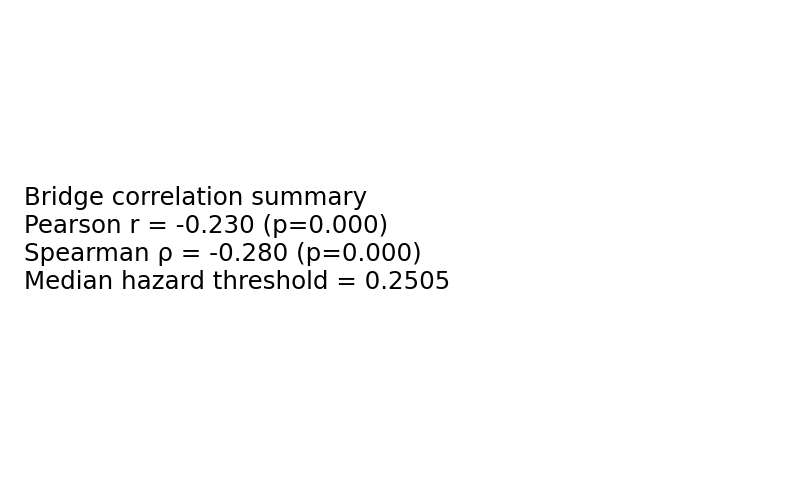
\includegraphics[width=0.5\linewidth]{../figures/fig4_bridge_correlation_summary.png}
  \caption{Correlation summary from `compute_bridge_metrics.py`.}
  \label{fig:bridge-summary}
\end{figure}

\section{Discussion}
We discuss parameter sensitivity (signature precision, hazard weighting), data dependencies (Valkey cache and OANDA fallbacks), and the limitations of current PlanBench coverage (synthetic traces remain statistically weak under permutation tests).

\section{Conclusion}
The native QFH/QBSA manifold is now integrated into the STM pipelines and makes it possible to compare planning and trading domains using a unified signal vocabulary. Future work will refine the bridge correlation and expand the FX dataset to capture regime changes.

\appendix
\section{Reproducibility}
All commands are executed from the project root (`/sep/score`) with the virtual environment at `score/.venv` activated.
The following script regenerates the native artefacts end-to-end:
\begin{verbatim}
# Build native bindings
python -m venv .venv
source .venv/bin/activate
python -m pip install --upgrade pip
pip install -e .[native]

# Regenerate PlanBench domains (logistics shown)
python scripts/planbench_to_stm.py \
  --input-root data/planbench_public \
  --domains logistics \
  --output output/planbench_by_domain/logistics \
  --use-native-quantum

# Enrich logistics features
python scripts/enrich_features.py \
  output/planbench_by_domain/logistics/invalid_state.json \
  --features logistics --use-native-quantum \
  --output output/planbench_by_domain/logistics/invalid_state_logistics_native.json

# Calibrate guardrail with native metrics
python scripts/calibrate_router.py \
  output/planbench_by_domain/logistics/invalid_state.json \
  --target-low 0.05 --target-high 0.07 \
  --domain-root output/planbench_by_domain/logistics \
  --dynamic-target 0.025 --dynamic-window 0.005 \
  --pvalue-threshold 0.05 --pvalue-metric min \
  --output analysis/router_config_logistics_invalid_native.json \
  --use-native-quantum

# Synthetic dataset
python scripts/experiments/qfh_synthetic.py \
  --output results/qfh_synthetic_native.json

# Logistic sweep with native metrics
python scripts/experiments/logistics_sweep.py \
  --state output/planbench_by_domain/logistics/invalid_state.json \
  --domain-root output/planbench_by_domain/logistics \
  --results-dir results/logistics_sweep_native \
  --summary-output results/logistics_sweep_summary_native.json \
  --use-native-quantum

# Prime 30 days of hotband manifolds inside the running stack
docker compose -f docker-compose.hotband.yml exec backend \
  python scripts/ops/prime_qfh_history.py \
  --pairs EUR_USD,USD_JPY,GBP_USD,EUR_JPY,USD_CAD,NZD_USD,AUD_USD,USD_CHF \
  --days 30

# Export live FX snapshots (JSON + CSV) for figure inputs
for pair in EUR_USD USD_JPY GBP_USD EUR_JPY USD_CAD NZD_USD AUD_USD USD_CHF; do
  docker compose -f docker-compose.hotband.yml exec backend \
    python scripts/ops/export_manifold_snapshots.py \
    --instrument "$pair" \
    --minutes $((30*24*60)) \
    --out output/manifolds_native/${pair}_snapshots.json;
done

# Whitepaper figures
python scripts/plot_whitepaper_figures.py \
  --sweep results/logistics_sweep_summary_native.json \
  --warmup-dir output/warmup/EUR_USD \
  --logistics-state output/planbench_by_domain/logistics/invalid_state_logistics_native.json \
  --synthetic results/qfh_synthetic_native.json \
  --planbench-native output/planbench_by_domain/logistics/gold_state_logistics_native.json \
  --fx-manifolds output/manifolds_native \
  --bridge-metrics docs/note/bridge_metrics.json \
  --outdir docs/figures \
  --note-dir docs/note
\end{verbatim}

\end{document}
